\chapter{Θεωρητικό Υπόβαθρο}
\label{chapter:theory}

Στο κεφάλαιο αυτό θα παρουσιαστούν εργαλεία που χρησιμοποιήθηκαν για την υλοποίηση του Συστήματος
Ενεργής Παρακολούθησης, καθώς και έννοιες και τεχνολογίες που αξιοποιήθηκαν για το σκοπό αυτό.

\section{Hypertext Transfer Protocol}
\label{section:http}

Το πρωτόκολλο επικοινωνίας HTTP (Hypertext Transfer Protocol) αποτελεί το πιο διαδεδομένο και ευρέως γνωστό
πρωτόκολλο στο χώρο του διαδικτύου. Αναπτύχθηκε από τους Tim Berners-Lee και την ομάδα του το 1990 και από τότε
έχει περάσει πολλές αλλαγές προκειμένου να μπορεί να ανταπεξέλθει στις ολοένα και συνεχώς αυξανόμενες ανάγκες του σήμερα.

Αποτελεί τη βάση κάθε μετάδοσης πληροφορίας στο διαδίκτυο. Στηρίζεται στην επικοινωνία δύο υπολογιστών, ενός που κάνει τα αιτήματα (client)
και ενός που απαντά σε αυτά (server). Στο τέλος της επικοινωνίας στην μεριά του παραλήπτη θα υπάρχει ανακατασκευασμένο
ένα ολοκληρωμένο αρχείο, από τα διάφορα υπο-αρχεία που μαζεύτηκαν, που μπορεί να είναι αρχεία ήχου, εικόνας, video.
Τα αιτήματα αυτού που ξεκινάει την επικοινωνία ονομάζονται requests, ενώ οι απαντήσεις του αποστολέα responses.

Η βασική δομή ενός http αιτήματος, η οποία φαίνεται και στο \autoref{fig:http_request}, περιληπτικά περιλαμβάνει τη μέθοδο (method) του αιτήματος, που περιγράφει
τη βασική λειτουργία του, το μονοπάτι (path) στο οποίο θα επικοινωνήσει με τον server, την έκδοση του πρωτοκόλλου που 
θα χρησιμοποιηθεί και τέλος headers προκειμένου να κρίνει ο server αν πρέπει να απαντήσει ή όχι πίσω στον client

\begin{figure}[!ht]
	\centering
	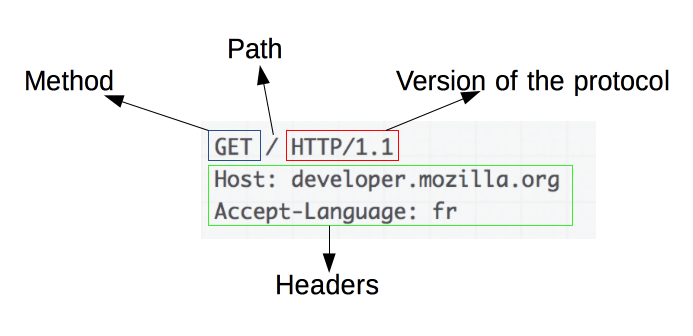
\includegraphics[width=0.7\textwidth]{./images/chapter2/http_request.png}
	\caption[Βασική Δομή ενός αιτήματος http]{Βασική Δομή ενός αιτήματος http}
	\label{fig:http_request}
\end{figure}

\subsection{Μέθοδοι}
\label{subsec:http_methods}

Πιο συγκεκριμένα οι βασικές μέθοδοι που παρέχει το http και οι συνήθεις λειτουργίες τους είναι οι εξής:

\begin{itemize}
	\item \textbf{GET}: παίρνει πληροφορία από τον server
	\item \textbf{POST}: υποβάλλει πληροφορία, προκαλώντας αλλαγές στον τρόπο λειτουργίας του server. Σχετίζεται συχνά με τη δημιουργία πληροφορίας που προηγουμένως δεν υπήρχε 
	\item \textbf{PUT}: όπως και πριν στέλνει πληροφορία στον παραλήπτη υπολογιστή, αλλά αυτή τη φορά επηρεάζει πόρους που ήδη υπήρχαν στο σύστημα. Σχετίζεται συχνά με την τροποποίηση ήδη υπάρχουσας πληροφορίας
	\item \textbf{DELETE}: διαγράφει από το σύστημα του server το συγκεκριμένο πόρο.
\end{itemize}

Αξίζει να σημειωθεί ότι πέρα από τις τέσσερις αυτές βασικές μεθόδους υπάρχουν και άλλες όπως είναι 
η \textbf{PATCH} που αποτελεί ειδική περίπτωση της PUT, η \textbf{HEAD} που αποτελεί ειδική περίπτωση της GET,
καθώς και άλλες που σχετίζονται με τη σύνδεση μεταξύ server και client. Αυτές είναι οι \textbf{CONNECT}, \textbf{OPTIONS} και \textbf{TRACE}.
Καθώς όμως, οι υπόλοιπες αυτές οι μέθοδοι, δεν χρησιμοποιούνται τόσο συχνά στην πράξη, δεν θα αναλυθούν περαιτέρω.

\subsection{Εκδόσεις HTTP}
\label{subsec:http_versions}

Η πρώτη έκδοση του HTTP, παρόλλο που δεν είχε κάποια συγκεκριμένo τίτλο, εκ των υστέρων ονομάστηκε 
HTTP/0.9. Αποτελεί την πιο απλή έκδοση του πρωτοκόλλου. Δεν υποστηρίζονταν headers και κωδικοί κατάστασης (status codes).
Εξυπηρετούσε μόνο GET αιτήματα και η μοναδική απάντηση που μπορούσε να επιστρέψει ήταν hypertext αρχεία. Kάθε φορά που ο server ανταποκρινόταν και έστελνε
απάντηση, η επικοινωνία με τον client έκλεινε κατευθείαν.

Στη συνέχεια και με την ανάπτυξη του διαδικτύου προστέθηκαν και άλλες λειτουργίες. Πέριξ του 1996,
με τη επόμενη έκδοση του πρωτοκόλλου (HTTP/1.0) τα αιτήματα πλέον συνοδεύονταν από headers, μεταπληροφορία σχετικά
με τη κατάσταση του αιτήματος, τον τύπο της πληροφορίας που περιμένουμε να έρθει (stylesheets, media, hypertext) καθώς και 
την έκδοση του HTTP που χρησιμοποιήθηκε στη συγκεκριμένη επικοινωνία. Επιπλέον πέρα από τη GET μέθοδο υπάρχει η
δυνατότητα για POST και PUT, δημιουργία και τροποποίηση πληροφορίας δηλαδή.

Στη συνέχεια το HTTP/1.1 προσπαθεί να βελτιώσει τις ήδη υπαρχουσες δυνατότητες κάνοντας την επικοινωνία
μεταξύ server και client πιο αποδοτική. Αντί να κλείνει η επικοινωνία μετά από κάθε μήνυμα, η σύνδεση παραμένει
ανοιχτή γλιτώνοντας έτσι μία σταθερή καθυστέρηση που υπήρχε σε κάθε αίτημα

Φτάνοντας στο σήμερα, μιλάμε για το HTTP/2.0 \cite{http2}. Αξιοποιώντας το πρωτόκολλο Speedy (SPDY) που αναπτύχθηκε κάποια χρόνια πριν
την κυκλοφορία του, και κτίζοντας πάνω σε αυτό, κατάφερε να μειώσει τους χρόνους επικοινωνίας server-client.
Μερικοί από τους τρόπους που επιτυγχάνεται αυτό είναι η μετατροπή του http από text πρωτόκολλο, σε δυαδικό (binary protocoll), επιτρέποντας έτσι χρήση καλύτερων
και αποδοτικότερων τεχνικών επικοινωνίας. Επιπλέον συμπιέζει τους headers (header compression) καθώς αποτελούν πληροφορία που
επαναλαμβάνεται όταν τα αιτήματα στον server είναι συνεχή. Ο server ακόμα, αποκτά έναν μηχανισμό (server-push) που του
επιτρέπει να προωθεί πληροφορία στον client (στην cache του client συγκεκριμένα), που δεν έχει ζητήσει ακόμα, αλλά βάση αυτού
που αιτήται, μάλλον θα ζητήσει εντός της ιδίας συνεδρίας.

Τέλος, πρέπει να αναφερθούμε στην τελευταία, αν και όχι ακόμα ευρέως διαδεδομένη, έκδοση HTTP/3.0. H βασική διαφορά με τους
πρωκατόχους του είναι ότι αλλάζει το πρωτόκολλο επικοινωνίας που χρησιμοποιεί όλα αυτά τα χρόνια, από TCP (Transfer Communication Protocoll) σε
έναν συνδυασμό UDP (User Datagram Protocoll) και QUIC (Quick UDP Internet Connections), μίας νέας τεχνολογίας που λύνει το πρόβλημα και βελτιστοποιεί τόσο το πρόβλημα 
της ασφάλειας των επικοινωνιών (TLS handshakes), όσο και της απώλειας πληροφορίας που μπορεί να υπήρχε λόγω UDP, πρωτοκόλλου που είναι γνωστό
για την ταχύτερη απόδοσή του σε σχέση με το TCP, αλλά και το γεγονός ότι είναι πιο επιρρεπές σε σφάλματα. Η νέα αυτή έκδοση από τα αποτελέσματα 
του \cite{http3} φαίνεται να έχει ήδη καλύτερους χρόνους σε σχέση με τις παλαιότερες εκδόσεις και ήδη το 28\% του διαδικτύου αξιοποιεί τις δυνατότητές του. 


\subsection{Κωδικοί Κατάστασης}
\label{subsec:http_status_codes}

Οι κωδικοί κατάστασεις (status codes) αποτελούν μέρος της απάντησης του server. Επιτρέπουν στον χρήστη να καταλάβει με μία ματιά αν το αίτημα που έχει κάνει έχει επιστρέψει σωστά, ή έχει γίνει κάποιο λάθος στη μεριά του server.
Υπάρχουν πέντε μεγαλύτερες κατηγορίες που στεγάζουν όλες τις υποπεριπτώσεις αυτών. Πιο συγκεκριμένα:

\begin{itemize}
	\item \textbf{Εύρος 100-199}: Υποδηλώνουν ενημερωτική απάντηση σχετικά με τη λειτουργία του server
	\item \textbf{Εύρος 200-299}: Επιτυχή αιτήματα. 
	\item \textbf{Εύρος 300-399}: Υποδηλώνουν την ανακατεύθυνση του μηνύματος του client. Συνήθως συνοδεύονται από το νέο url στο οποίο πρέπει να αποσταλλεί το αίτημα
	\item \textbf{Εύρος 400-499}: Ανεπιτυχές αίτημα, που οφείλεται στον client. Ένα σύνηθες παράδειγμα είναι η αίτηση πρόσβασης σε προστατευόμενους πόρους χωρίς κάποιου είδους αυθεντικοποίηση, ή χωρίς τα σωστά στοιχεία για αυθεντικοποίηση
	\item \textbf{Εύρος 500-599}: Ανεπιτυχές αίτημα, που οφείλεται στον server. 
\end{itemize}
\section{API}
\label{section:api}

Ένα ακόμα πολύ σημαντικό συστατικό του διαδικτύου αποτελούν οι Διεπαφές Εφαρμογών Προγραμμάτων (Application Programming Interfaces - APIs).
Πρόκειται για το σύνολο των ορισμών, κανόνων και πρωτοκόλλων για τη δημιουργία και ενσωμάτωση μίας
εφαρμογής. Ουσιαστικά λειτουργεί ως το συμβόλαιο μεταξύ ενός συστήματος παροχής υπηρεσίας και του
χρήστη του συστήματος αυτού, καθορίζοντας την απαραίτητη πληροφορία που απαιτεί για να λειουργήσει σωστά
ο server αλλά και αντίστροφά, καθορίζοντας την απαραίτητη πληροφορία που απαιτεί ο client στην απάντηση
που θα του επιστραφεί.

Είναι εμφανές λοιπόν ότι σε κάθε περίπτωση, αν θέλει κανείς να αλληλεπιδράσει με κάποιο σύστημα
είτε για να αντλήσει πληροφορία, είτε για να στείλει πληροφορία (αποθήκευση ή τροποποίηση ήδη υπάρχουσας)
θα πρέπει να υπάρχουν κανόνες που ορίζουν και καθιστούν πιο εύκολη και απλή την επικοινωνία αυτή.

H έννοια του api δεν περιορίζεται φυσικά μόνο στο πλαίσιο του διαδικτύου, αλλά σε όλων των ειδών
εφαρμογές που υπάρχει επικοινωνία ενός κεντρικού σημείου (server) με κάποιον χρήστη (client) που θέλει να
κάνει χρήση των υπηρεσιών που αυτό προσφέρει.

Όσων αφορά τη διαθεσιμότητα και ασφάλεια των API, μπορούμε να διακρίνουμε τις εξής κατηγορίες:

\begin{itemize}
	\item \textbf{Ανοιχτά (Open):} Σε αυτού του τύπου διεπαφών λογισμικού, έχει ελεύθερη πρόσβαση ο καθένας,
		χωρίς να απαιτείται κάποια παραπάνω πληροφορία που αφορά την αυθεντικοποίηση ή ταυτοποίηση του χρήστη.
		Επειδή ακριβώς η πληροφορία που παρέχεται (ανοιχτά) έιναι τεράστια, χρησιμοποιούνται πολύ
		συχνά σε έρευνες, όπως η \cite{open_restful_api_analysis} που αξιοποιεί ελεύθερα προσβάσιμους
		πόρους για να αναλύσει τα πιο διαδεδομένα APIs. 
	\item \textbf{Δημόσια (Public):} Μοιάζουν πολύ με τα \textbf{Ανοιχτού Τύπου API}, με τη μόνη διαφορά, τον περιορισμό
		πρόσβασης σε ορισμένα σημεία που απαιτούν κλειδιά προκειμένουν να γίνει, σε αντίθεση με πριν, αυθεντικοποίηση και ταυτοποίηση. 
	\item \textbf{Ιδιωτικά (Private):} Αφορούν διεπαφές λογισμικού που αναπτύσσονται και χρησιμοποιούνται μόνο εντός ενός κλειστού
		πλαισίου, όπως θα μπορούσε να είναι μία επιχείρηση ή κάποιο πανεπιστήμιο που παρέχει ορισμένες υπηρεσίες μόνο εντός του χώρου του.
		Πολλές φορές στη βιβλιογραφία αναφέρονται και ως \textbf{Εσωτερικά (Internal APIs).}
	\item \textbf{Εταιρικά (Partner):} Είναι περιορισμένα στο πλήθος χρηστών που έχουν πρόσβαση σε αυτό. Χρησιμοποιούνται
		για επικοινωνία μεταξύ συστημάτων εταιριών/επιχειρήσεων για την ανάπτυξη και αξιοποίηση εφαρμογών και υπηρεσιών.
		Συνήθως η ασφάλεια σε όλες αυτές τις αλληλεπιδράσεις είναι αρκετά πιο αυστηρή.
	\item \textbf{Σύνθετα (Composite):} Συνδυάζουν περισσότερα από ένα API αιτημάτων σε ένα, κάνοντας έτσι 
		την επικοινωνία πιο αποδοτική (κερδίζοντας χρόνο από πολλά διαδοχικά APIs).
\end{itemize}

Αξίζει να σημειωθεί σε αυτό το σημείο ότι ο τρόπος δημιουργίας, η δομή, καθώς και τα πρωτόκολλα που χρησιμοποιούν τα διαφόρα APIs που υπάρχουν στο διαδίκτυο
δεν είναι πάντα κοινά. Yπάρχουν κάποιες γνωστές αρχιτεκτονικές και πρωτόκολλα, όπως θα δούμε και στη συνέχεια, που πέρα από τη δομή
των συστημάτων παρέχουν και κανόνες "Καλύτερων Πρακτικών" (Best Practices). Οι πιο γνωστές αριχτεκτόνικές
παρατίθενται στη συνέχεια:

\begin{itemize}
	\item \textbf{SOAP (Simple Object Access Protocol):} Χρησιμοποιούνταν ευρέως στο παρελθόν πριν την εμφάνιση του REST.
		Η επικοινωνία μεταξύ server και client επιτυγχάνεται με την αποστολή αρχείων XML.
	\item \textbf{RPC (Remote Procedure Call):} Αποτελεί πρωτόλλο επικοινωνίας που επιτρέπει σε ένα σύστημα (client) να καλεί διαδικασίες (procedures)
		ή συναρτήσεις σε ένα άλλο σύστημα (server) είτε αυτά είναι στο ίδιο δίκτυο, είτε απομακρυσμένα. Σκοπός είναι να
		κάνει τα δύο συστήματα να επικοινωνούν σαν να βρίσκονται στο ίδιο υπολογιστικό σύστημα. Επιγραμματικά η διαδικασία
		επικοινωνίας δύο συστημάτων ξεκινάει με ένα αίτημα στον server να εκτελέσει κάποια συγκεκριμένη λειτουργία, παρέχοντας
		ορίσματα που ίσως χρειαστούν για αυτό. Ο server τέλος επιστρέφει την απάντηση της παραπάνω διαδικασίας στον client. Σήμερα το πρωτόκολλο αυτό
		χρησιμοποιείται σε διάφορες εφαρμογές και αναπτύσσονται μάλιστα συνεχώς, σύχρονες τεχνολογίες που, πατώντας πάνω στη βασική λειτουργία
		του πρωτοκόλλου, κάνουν περαιτέρω βελτιστοποιήσεις (gRPC).
	\item \textbf{REST (Representational State Transfer)}: Η πιο διαδεδομένη μορφή API στο διαδίκτυο. Η λειτουργία του είναι απλή. Η χρήστης στέλνει αίτημα σε ένα
		απομακρυσμένο σύστημα (server). Το σύστημα αντιδράει, και βάσει των δεδομένων που του στέλνει ο χρήστης, τρέχει διαδικασίες ώστε να παράξει το
		επιθυμητό αποτέλεσμα, το οποίο τέλος αποστέλλει στον client.
	\item \textbf{Websocket}: Αποτελεί πρωτόκολλο που επιτρέπει την αμφίδρομη επικοινωνία μεταξύ client και server. Σε αντίθεση με το REST API, που κάθε φορά
		που γίνεται ένα αίτημα στον server πρέπει να αποστέλλονται οι κατάλληλοι headers και να γίνεται η κατάλληλη σύνδεση μεταξύ των δύο συστημάτων, με τη χρήση των websockets
		η σύνδεση αυτή εκτελείται μόνο μία φορά στο αρχικό αίτημα που αποστέλλεται. Αξίζει να σημειωθεί ακόμα ότι θεωρείται ιδανικό για εφαρμογές που απαιτούν άμεση ενημέρωση \cite{websockets} (real-time-applications)
		τόσo για τον προαναφερθέντα λόγο, βάσει του οποίου μειώνεται δραστικά ο χρόνος επικοινωνίας μεταξύ των εμπλεκόμενων, όσο και για το γεγονός ότι
		μηνύματα μπορούν να σταλούν και από τη μεριά του client προς τον server αλλά και το ανάποδο (server σε client) χωρίς να χρειάζεται να γίνει κάποιο αίτημα πρώτα.
\end{itemize}

\subsection{RESTful API}
\label{subsec:rest_api}

Πρόκειται για ένα τύπο αρχιτεκτονικής λογισμικού για APIs, που αποτελείται από κατευθυντήριες γραμμές και βέλτιστες πρακτικές για τη δημιουργία επεκτάσιμων εφαρμογών στο διαδίκτυο.
Προτάθηκε το 2000, από τον Thomas Fielding \cite{rest_proposal}, σαν ένας τρόπος για να κατευθύνει την ανάπτυξη εφαρμογών 
προκειμένου να υπάρχει ένα κοινός τρόπος "γραφής", ώστε να υπάρξη εξέλιξη στον τομέα αυτό ακόμα πιο γρήγορα και οργανωμένα.  
Το δομικό συστατικό του είναι το πρωτόκολλο HTTP που χρησιμοποιεί για να πραγματοποιεί κλήσεις μεταξύ συστημάτων.

Όπως προαναφέρθηκε ο τρόπος λειτουργίας στην απλούστερη έκδοσή του ξεκινάει με ένα αίτημα κάποιου χρήστη
σε ένα σύστημα της επιλογής του, παρέχοντας την απαραίτητη πληροφορία προκειμένου ο server να μπορέσει να αναταποκριθεί επιτυχώς.
Έπειτα, και αφού το σύστημα διεκπεραιώσει όλες τις εσωτερικές λειτουργίες του, απαντά μεταφέροντας πίσω στον χρήστη
την επιθυμητή πληροφορία και ενημερώνοντας τον σχετικά με την κατάσταση του αιτήματος του (σε περίπτωση που κάτι πήγε λάθος ο χρήστης
θα πρέπει να ενημερώνεται αναλόγως).

Ο βασικός τρόπος αλληλεπίδρασης με τους πόρους του συστήματος θα πρέπει να γίνεται
μέσα από τις τέσσερις βασικές μεθόδους του HTTP (\textbf{GET, POST, PUT, DELETE}), χωρίς αυτό να απαγορεύει
τη χρήση των υπόλοιπων. Κάθε σύστημα θα πρέπει τυπικά να υποστηρίζει CRUD λειτουργίες (Create, Read, Update, Delete). Αυτές σχετίζονται
με την ύπαρξη μεθόδων εντός του συστήματος που θα επιτρέπουν τη δημιουργία δεδομένων και την τροποποίηση, ανάγνωση, και διαγραφή ήδη υπάρχουσας πληροφορίας. 

Για να χαρακτηριστεί ένα API ώς RESTful θα πρέπει να ικανοποιεί τα παρακάτω, ενώ
στο \autoref{fig:rest_principles} μπορούμε να τα δούμε σε ένα γενικότερο πλαίσιο:

\begin{itemize}
	\item \textbf{Client-Server:} Τα δύο αυτά υπολογιστικά συστήματα θα πρέπει να είναι ανεξάρτητα.
		Πρακτικά αυτό σημαίνει ότι ο client θα ασχοληθεί αποκλειστικά και μόνο με το κομμάτι παρουσιάσης της πληροφορίας, που του παρέχει ο server,
		στον χρήστη μέσα από διεπαφές γραφικού χαρακτήρα, ενώ ο server θα εκτελεί μόνο λειτουργίες που αφορούν την δημιουργία, τροποποίηση και διαγραφή των πόρων του
		συστήματος. Με αυτό τον διαχωρισμό πλέον o client είναι πιο ελαφρής, καθώς διαχειρίζεται μόνο πληροφορία που του έρχεται έτοιμη από το σύστημα,
		και ο server μπορεί να κάνει πιο εύκολα scaling.
	\item \textbf{Cacheable:} ο client θα πρέπει να αποθηκεύει προσωρινά (cache) τις
		απαντήσεις που λαμβάνει από τον server για την αποφυγή συνεχών επαναλαμβανόμενων αιτημάτων, βελτιώνοντας
		έτσι την απόδοση του συστήματος.
	\item \textbf{Stateless:} Η πληροφορία της κατάστασης του συστήματος δεν θα πρέπει να αποθηκεύεται
		αλλά κάθε αίτημα θα πρέπει να περιέχει την απαραίτητη πληροφορία για να εκτελεστεί από τη μεριά του server.
		Η πληροφορία αυτή μπορεί να αποτελεί μέρος του ίδου του url, του body, των headers ή του query.
	\item \textbf{Πολυεπίπεδο Σύστημα (Layered System):} Τα υπολογιστικά συστήματα που συμμετέχουν στη διαδικασία αυτή δεν
		θα πρέπει να γνωρίζουν αν είναι άμεσα συνδεδεμένα μεταξύ τους ή υπάρχουν ενδιάμεσοι κόμβοι που παρεμβάλλονται.
		Το σύστημα θα πρέπει να λειτουργεί δίχως να έχει επίγνωση των γειτόνων του, περιμένοντας απλά την κατάλληλη πληροφορία για να
		λειτουργήσει, τόσο από τη μεριά του server όσο και από τη μεριά του client.
\end{itemize}

\begin{figure}[!ht]
	\centering
	\makebox[\textwidth][c]{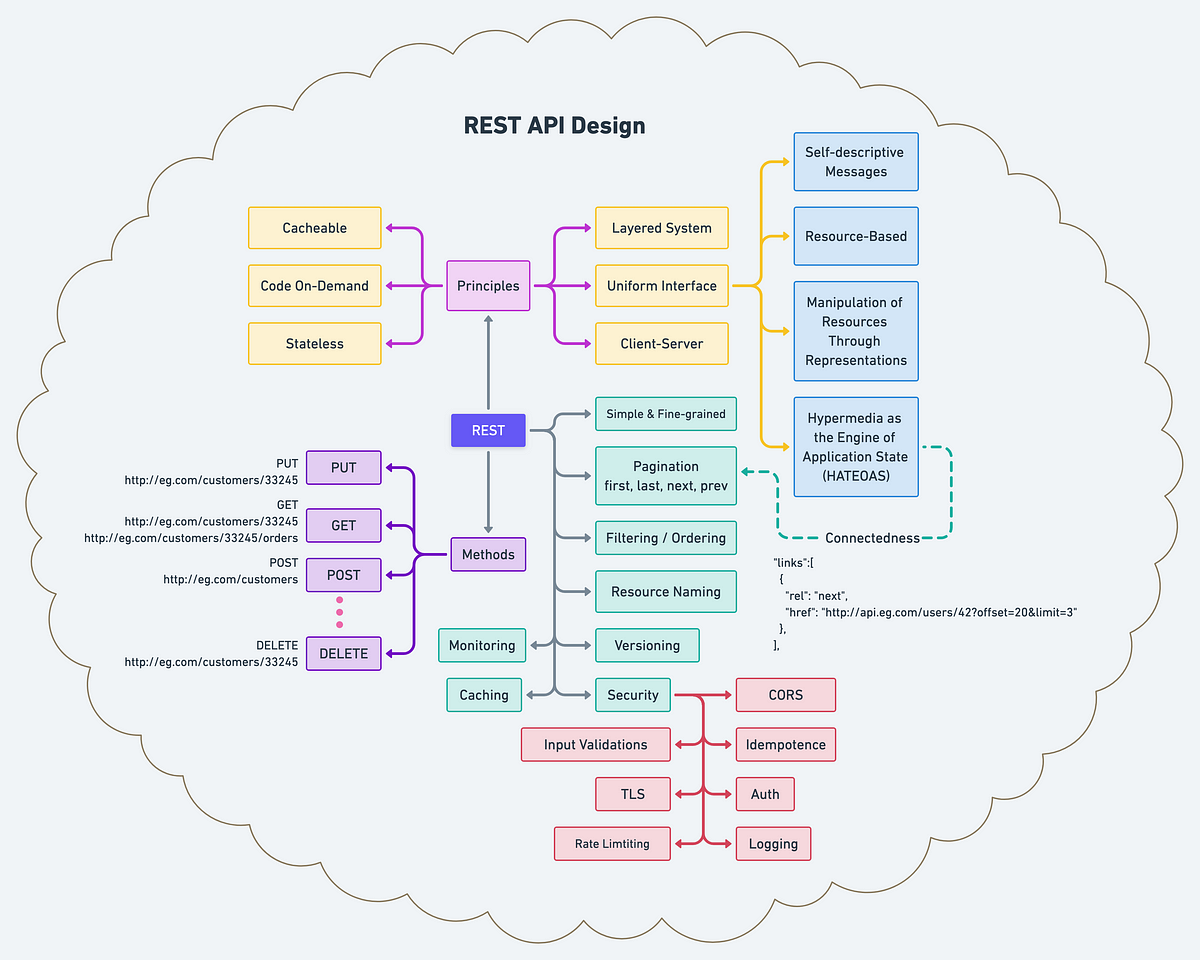
\includegraphics[width=1\textwidth]{./images/chapter2/rest_principles.png}}%
	\caption[Αρχές και Καλές Πρακτικές Σχεδίασης REST API]{Αρχές και Καλές Πρακτικές Σχεδίασης REST API}
	\label{fig:rest_principles}
\end{figure}
\section{Avro}
\label{section:avro}

Αποτελεί μία μορφή αποθήκευσης πληροφορίας που λόγω της υλοποίησης του παράγει αρχεία
πολύ μικρότερου μεγέθους από ότι θα αναμέναμε σε άλλου είδους μορφές αρχείων. Αναπτύχθηκε αρχικά για
τη για την αποθήκευση και τη μετάδοση πληροφορίας εντός του framework Apache Hadoop, αλλά έκτοτε
έχει χρήση και σε πλήθος άλλων εφαρμογών. Διαθέτει διεπαφές (API) που επιτρέπουν την ενσωμάτωση της τεχνολογίας αυτής σε
προγμάμματα γραμμένα σε πλήθος γλωσσών, μερικές εκ των οποίων είναι οι Java, C/C++/C\#, Python, PHP, Ruby, Rust και JavaScript.

Η βασικότερη διαφορά μεταξύ αρχείων avro και άλλων αρχείων αποθήκευσης πληροφορίας, όπως είναι τα JSON αρχεία
που αποτελούν τον πιο διαδεδομένο τρόπο αποθήκευσης στο χώρο του διαδικτύου, είναι το γεγονός
ότι διαθέτουν το schema των δεδομένων (data schema definition) που περιέχουν. Ξέροντας τη μορφή της προς αποθήκευσης πληροφορίας
καταφέρνουν να γλιτώσουν χώρο στο τελικό προϊόν. Αυτό σε συνδύασμό με το γεγονός ότι η πληροφορία αποθηκεύεται
συμπιεσμένη σε δυαδική μορφή (binary format) την καθιστά αρκετά σημαντική σε περιπτώσεις που έχουμε μεγάλο πλήθος πληροφορίας
που θέλουμε να αποθηκεύσουμε.

Τα βασικότερα πλεονεκτήματα του παρατίθενται στη συνέχεια ενώ η δομή ενός τέτοιου αρχείου φαίνεται στο \autoref{fig:avro_file_format}:

\begin{itemize}
	\item Είναι χρήσιμος για την μετάδοση πληροφορίας, καθώς η αποθηκευμένη πληροφορία είναι
		αρκετά συμπυκνωμένη.
	\item Επιτρέπει την τροποποίηση και εξέλιξη του σχήματος των δεδομένων (schema evolution), δίνοντας
		τη δυνατότητα για αλλαγές και data migration που πολλές φορές καθίστανται επιτακτικά 
		στη διάρκεια ζωής ενός προγράμματος που συνεχώς εξελίσσεται.
	\item Διαθέτει πλήθος τύπων δεδομένων απλών (primitive) και σύνθετων (complex) που μπορούν να χρησιμοποιηθούν
		\begin{itemize}
			\item Primitive: boolean, int, long, float, double, bytes, string
			\item Complex: record, enum, array, map, fixed, union 
		\end{itemize}
	\item Το schema εμπεριέχεται σε κάθε αρχείο. Κάνοντας χρήση αυτού κάθε χρήστης που έχει
		πρόσβαση σε ένα τέτοιο αρχείο μπορεί να διαβάσει τα περιεχόμενα του (εξαρχής binary, μη αναγνώσιμών από τον άνθρωπο)
		χωρίς να ξέρει από πριν τη μορφή της πληροφορίας. 
\end{itemize}


\begin{figure}[!ht]
	\centering
	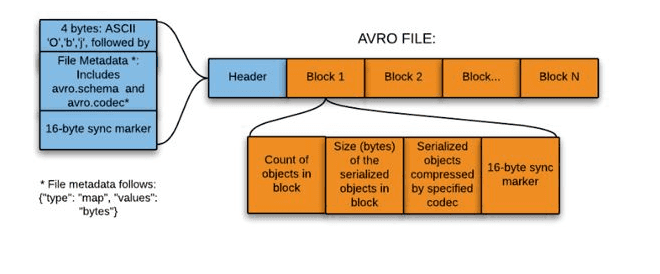
\includegraphics[width=0.7\textwidth]{./images/chapter2/avro_file_format.png}
	\caption[Δομή ενός avro αρχείου]{Δομή ενός avro αρχείου}
	\label{fig:avro_file_format}
\end{figure}
\break
\section{Στατιστικές μετρικές}
\label{section:statistics}

Στην υποενότητα αυτή θα δούμε τον τρόπο υπολογισμού μερικών κλασικών μετρικών της στατιστικής
που χρησιμοποιούνται για την εξαγωγή συμπερασμάτων στο σύνολο των δεδομένων που αποθηκεύουμε.
Σε όλους τους παρακάτω τύπους έχουμε δεδομένα $x_i$ όπου, $i = 0, ..., k$

\begin{enumerate}
	\item \textbf{Αριθμητική Μέση Τιμή}: Αποτελεί μία από τις πιο βασικές μετρικές που χρησιμοποιείται ευρέως σε στατιστικές μελέτες.
		Περιγράφει την τάση του εκάστοτε συνόλου δεδομένων που μελετάμε να κυμαίνεται γύρω από μία τιμή.
	      \begin{equation}
		      mean(x) = \frac{\sum_{n = 1}^{k} x_n}{k}
	      \end{equation}
	\item \textbf{Διάμεσος}: Είναι η τιμή που διαχωρίζει το υψηλότερο μισό από το κάτω μισό ενός διατεταγμένου συνόλου δεδομένων 
	      \begin{equation}
		      median(x) =
		      \begin{cases}
			      x_{\frac{n + 1}{2}}                             & \text{για n περιττό}
			      \\[10pt]
			      \frac{x_{\frac{n}{2}} + x_{\frac{n}{2} + 1}}{2} & \text{για n ζυγό}
		      \end{cases}
	      \end{equation}
	\item \textbf{Τυπική Απόκλιση Πληθυσμού}: Περιγράφει το κατά πόσο απέχουν το σύνολο των δεδομένων, κατά μέση τιμή, από τον \textbf{Μέσο Όρο}
	      \begin{equation}
		      std(x) = \sqrt{\frac{\sum_{i = 1}^{n} (x_i - mean(x))^2}{n - 1}}
	      \end{equation}
	\item \textbf{Τεταρτημόρια}: Όπως και η διάμεσος αποτελούν τις τιμές που διαχωρίζουν το σύνολο, των
		  διατεταγμένων κατά αύξουσα σειρά, δεδομένων στο 25\% και 75\% αντίστοιχα  
	      \begin{equation}
				\begin{cases}
					q1(x) = mean(x_i) & \text{όπου i = 0, ...., k/2} \\
					q3(x) = mean(x_j) & \text{όπου j = k/2 + 1, ...., k}
				\end{cases}
	      \end{equation}
\end{enumerate}

\break
\section{Εργαλεία}
\label{section:tools}

Στην τελευταία υποενότητα αυτού του κεφαλαίου θα μιλήσουμε για τα εργαλεία που χρησιμοποιήθηκαν
για την υλοποίηση του συστήματος Αυτόματης Παρακολούθησης που υλοποιήσαμε στο πλαίσιο της διπλωματικής
αυτής εργασίας.

\subsection{Node.js}
\label{subsec:nodejs}

Είναι ένα περιβάλλον εκτέλεσης (runtime) της προγραμματιστικής γλώσσας JavaScript.
Πληθώρα μηχανικών λογισμικού το χρησιμοποιούνε σήμερα, για την γρήγορη και, σχετικά με άλλα εργαλεία,
εύκολη ανάπτυξη διαδικτυακών εφαρμογών. Η Node.js μάλιστα διαθέτει το δικό της package manager
(ΝPM - Node Package Manager), στον οποίο διαρκώς προστίθενται καινούργιες βιβλιοθήκες
από χρήστες για χρήστες. 

Είναι σχεδιασμένο για να μπορεί να χτίζει κλιμακούμενες (scalable) εφαρμογές, καθώς η αρχιτεκτονική του,
επιτρέπει τη σύνδεση πολλών εξωτερικών συστημάτων/χρηστών και την εξυπηρέτηση αυτών ταυτόχρονα. Κάθε φορά που γίνεται κάποια σύνδεση στην εφαρμογή και κατεπακόλουθω
κάποιο αίτημα στο σύστημα εκτελείται μία callback συνάρτηση προκειμένου να μπορέσει να απαντήσει πίσω.
Όσο το σύστημα δεν δέχεται αιτήματα "κοιμάται" και περιμένει το επόμενο που θα έρθει.

Όλα όσα προαναφέρθηκαν την καθιστούν κατάλληλη για τη δημιουργία συστημάτων server. Αξίζει να σημειωθεί μάλιστα ότι για το σκοπό
αυτό υπάρχουν πλήθος βιβλιοθηκών που παρέχουν έτοιμες συναρτήσεις και διεπαφές που κάνουν την διαδικασία ανάπτυξης ακόμα πιο εύκολη
και γρήγορη. Πολλές φορές μάλιστα, κάποιες βιβλιοθήκες πέρα από βοηθητικές συναρτήσεις και υπορουτίνες, επηρεάζουν τον τρόπο
σύγγραφής κώδικα, μέσα από APIs που παρέχουν. Αυτές χαρακτηρίζονται ως frameworks, και επιταχύνουν τόσο τη διαδικασία
ελέγχου (testing), όσο και τη διαδικασία ανάπτυξης (development) του λογισμικού. Μερικές από τα πιο γνωστά
backend framerworks είναι τα: Express, Jest, Koa, Socket.io, Meteor, Loopback

Τα παραπάνω σε συνδυασμό με το ότι η JavaScript είναι μία ευρέως διαδεδομένη και πολυχρησιμοποιούμενη γλώσσα
προγραμματισμού στο διαδίκτυο δίνει την ευκαιρία σε developers να αναπτύξουν μία εφαρμογή πλήρως
(frontend και backend) με τη χρήση ενός κοινού εργαλείου. Ένα τυπικό παράδειγμα εφαρμογής που μπορεί να
αναπτυχθεί με τον τρόπο αυτό φαίνεται στο \autoref{fig:nodejs_system}.

\begin{figure}[!ht]
	\centering
	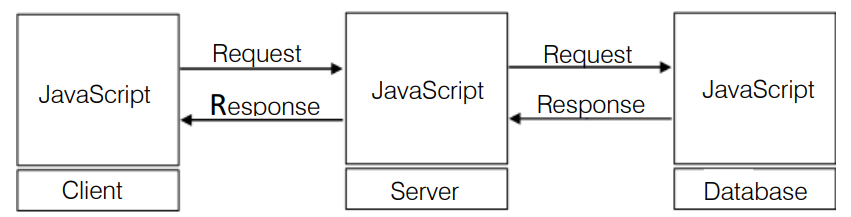
\includegraphics[width=0.8\textwidth]{./images/chapter2/javascript_end_to_end.png}
	\caption[Σχεδίαση συστήματος με χρήση Node.js]{Σχεδίαση συστήματος με χρήση Node.js \cite{nodejs_challenges_in_implementation}}
	\label{fig:nodejs_system}
\end{figure}

\subsection{PM2}
\label{subsec:pm2}

Η διαχείρηση διεργασιών (processes) που τρέχουν σε ένα υπολογιστικό σύστημα μπορεί να είναι δύσκολη
και αρκετά περίπλοκη για κάποιον που δεν διαθέτει μεγάλη πείρα σε αυτό τον τομέα. Το PM2 ή αλλιώς Process Manager 2,
αποτελεί ένα open source πρότζεκτ που κάνει την παραπάνω διαδικασία πιο απλή και κατανοητή, κερδίζοντας χρόνο
για τον developer που μπορεί να τον αξιοποιήσει για την ανάπτυξη εφαρμογών.

Με την έννοια διαχείρηση διεργασιών, αναφερόμαστε σε όλες εκείνες τις ενέργειες που σχετίζονται
με τον (πρόωρο ή όχι) τερματισμό και την παρακολούθηση ήδη υπάρχοντων διεργασιών (\autoref{fig:pm2_monitoring}), αλλά και τη δημιουργία καινούργιων.
Προγράμματα όπως το pm2 προσφέρουν ακόμα δυνατότητες όπως είναι η αυτόματη επανεκκίνηση διεργασιών σε περίπτωση σφάλματος
αποτρέποντας έτσι την ύπαρξη downtime των εφαρμογών που τρέχουμε.

Ένα από τα πιο χρήσιμα εργαλεία που παρέχει το PM2 είναι η λειτουργία cluster mode.
Αν και δεν αναφέρθηκε πιο πάνω ο συγκεκριμένος διαχειριστής διεργασιών εξειδικεύεται σε Node.js
εφαρμογές και στη διαχείρηση αυτών. Εξ ορισμού εφαρμογές γραμμένες σε JavaScript τρέχουν σε ένα thread
στο υπολογιστικό σύστημα που εκτελούνται. Χρησιμοποιώντας όμως το cluster mode, μπορούμε να
ξεκινήσουμε πολλαπλές διεργασίες που θα λειτουργούν ταυτόχρονα και θα μοιράζουν το φόρτο
κατάλληλα (load-balancing) ώστε το τελικό σύστημα να έχει καλύτερη απόδοση και να μπορεί να εξυπηρετεί 
περισσότερο κόσμο. 

\begin{figure}[!ht]
	\centering
	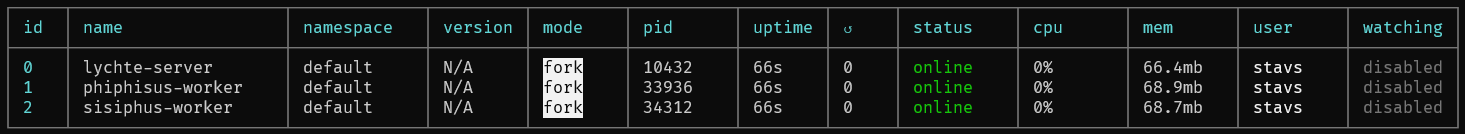
\includegraphics[width=1\textwidth]{./images/chapter2/pm2_monitoring.png}
	\caption[Παράδειγμα Παρακολούθησης διεργασιών με τη χρήση του PM2]{Παράδειγμα Παρακολούθησης διεργασιών με τη χρήση του PM2}
	\label{fig:pm2_monitoring}
\end{figure}

\subsection{MongoDB}
\label{subsec:mongodb}

H MongoDB αποτελεί μία Μη Σχεσιακή Βάση Δεδομένων (Non Relational Database), που χρησιμοποιεί documents,
για να αποθηκεύσει πληροφορία, αντί στήλες και γραμμές όπως θα είχαμε σε κλασσικές SQL βάσεις δεδομένων.
Είναι σχεδιασμένη για αποθήκευση δεδομένων μεγάλης κλίμακας και παράλληλη επεξεργασία δεδομένων μοιρασμένα
σε έναν μεγάλο αριθμό από servers. 

Τα documents που αναφέρθηκαν αποτελούν τον ακρογωνιαίο λίθο της Mongo, καθώς αποτελούν τη βασική μονάδα
της αποθηκευμένης πληροφορίας. Μορφοποιούνται ως BJSON (Binary JSON) και παρέχουν πληθώρα τύπων δεδομένων
που μπορείς να αποθηκεύσεις (string, integer, double, boolean, array, object, date, timestamp, null, binary). Κάθε βάση mongo μπορεί να περιέχει μία ή περισσότερες συλλογές (collections),
τα δεδομένα των οποίων πρέπει να υπακούουν στο ίδιο σχήμα (schema). Επειδή όμως η βάση αυτή παρέχει
δυνατότητες δυναμικού σχήματος (dynamic schema) μπορούμε να αποθηκεύουμε πληροφορία και να προσθέτουμε πεδία (fields)
που δεν είχαμε ορίσει από την αρχή δημιουργίας του συστήματος. \\

Μερικοί από τους λόγους που την επιλέξαμε είναι οι εξής:

\begin{itemize}
	\item \textbf{Document Oriented Storage}: η αποθήκευση και διαχείρηση των δεδομένων
		(στο πλαίσιο της εφαρμογής) είναι εύκολη καθώς στηρίζεται σε δεδομένα σε μορφή JSON.
	\item \textbf{Ευρετήρια (Indexes)}: Μπορείς κατά τη διαδικασία του στησίματος της βάσης (αλλά και μετέπειτα)
		να ορίσεις ευρετήρια σε πεδία που χρησιμοποιούνται συχνά σε queries προκειμένου
		να βελτιώσεις την απόδοση του συστήματος στο σύνολο. Όσο πιο γρήγορη είναι βάση, τόσο
		καλύτερη θα είναι η ανταπόκριση του συστήματος. 
	\item \textbf{Ομοιοτυπία (Replication) και μεγάλη Διαθεσιμότητα}: Δημιουργώντας πολλαπλά αντίτυπα των αποθηκευμένων δεδομένων	
		σε περισσότερο από έναν servers, μπορούμε να είμαστε σίγουροι ότι θα έχουμε πρόσβαση στην
		πληροφορία ακόμα και αν η κίνηση (data traffic) της εφαρμογής αυξηθεί.
	\item \textbf{Αυτόματο sharding}: Διασπώντας την αποθηκευμένη πληροφορία και έχοντας τμήματα αυτής σε διαφορετικούς server
		μας δίνεται η δυνατότητα να κάνουμε οριζόντιο scaling πολύ πιο εύκολα. 
	\item \textbf{Εύκολο ενσωμάτωση}: Η mongo διαθέτει βιβλιοθήκες στο περιβάλλον του node.js που καθιστούν
		τη χρήση και το στήσιμό της πολύα απλό. Πέρα από τη mongo, την επίσημη βιβλιοθήκη που υπάρχει,
		διατίθεται και η mongoose που αποτελεί μία Object Data Modelling (ODM) βιβλιοθήκη για τη Mongo και τη nodejs (\autoref{fig:mongoose}) 
\end{itemize}

\begin{figure}[!ht]
	\centering
	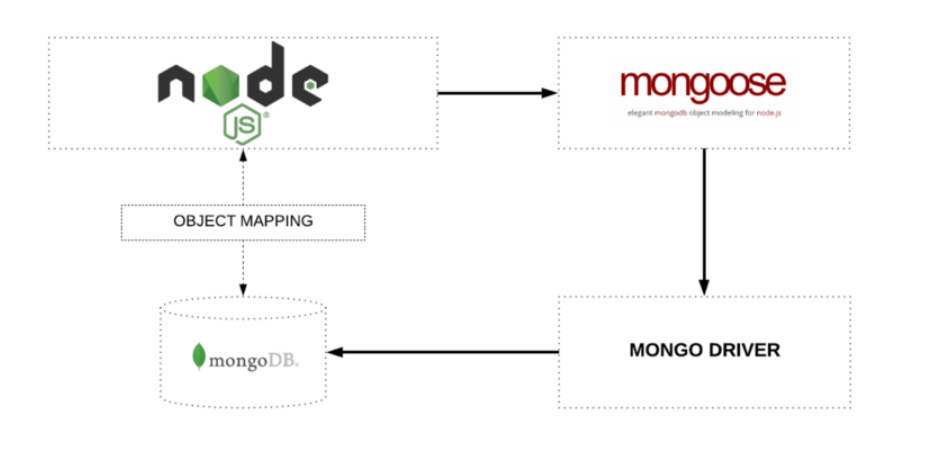
\includegraphics[width=0.8\textwidth]{./images/chapter2/mongoose.png}
	\caption[H mongoose λειτουργεί ώς ένα abstract layer μεταξύ της Node και των driver της mongo προκειμένου η επικοινωνία μεταξύ των δύο να γίνεται πιο εύκολα]
	{H mongoose λειτουργεί ώς ένα abstract layer μεταξύ της Node και των driver της mongo προκειμένου η επικοινωνία μεταξύ των δύο να γίνεται πιο εύκολα}
	\label{fig:mongoose}
\end{figure}

\break

\subsection{Google Cloud Storage}
\label{subsec:gcloud}

Πέρα από την κλασική βάση δεδομένων που προαναφέραμε θέλουμε να αποθηκεύουμε ιστορικά δεδομένα,
δεδομένα δηλαδή που δεν θα δείχνουμε άμεσα στον χρήστη, αλλά θα κρατάμε για να υπολογίζουμε μετρικές
και στατιστικά σημαντικά αποτελέσματα στο σύνολο όλης της μέχρι τώρα αποθηκευμένης πληροφορίας.

Σε αυτό λοιπόν το σημείο έρχεται το Google Cloud Storage (GCP), το οποίο παρέχει μεταξύ άλλων δυνατότητες
Αποθήκευσης Αρχείων (File Storage). Τα δεδομένα αυτά δεν χρειάζεται να υπακούουν σε κάποιο σχήμα
ενώ παράλληλα ο τρόπος αρχειοθέτησης των δεδομένων ταυτίζεται με ένα κλασικό σύστημα αρχείων
ενός υπολοσιστικού συστήματος. Διαθέτει paths και τύπους αρχείων όπως ακριβώς και οι υπολογιστές και όλες οι
συσκευές που χρησιμοποιούμε. Για να διαβάσεις κανείς πληροφορία, χρειάζεται να ξέρει μόνο το μονοπάτι που οδηγεί
στο επιθυμητό αρχείο καθώς και τη μορφή αυτού. Οι υποστηριζόμενοι τύποι αρχείων μέχρι τώρα είναι οι εξής:

\begin{itemize}
	\item Binary
	\item Flat
	\item JSON
	\item Avro
	\item Parquet
\end{itemize}

